%%%% Better Poster latex template example v1.0 (2019/04/04)
%%%% GNU General Public License v3.0
%%%% Rafael Bailo
%%%% https://github.com/rafaelbailo/betterposter-latex-template
%%%%
%%%% Original design from Mike Morrison
%%%% https://twitter.com/mikemorrison

\documentclass[poster, fleqn]{betterposter}
\usepackage[colorlinks=true, urlcolor=white]{hyperref}
\usepackage{tikz}
\usepackage{setspace}
\usepackage{pgf}
\usepackage[most]{tcolorbox} %% colored boxes

%%%%%%%%%%%%%%%%%%%%%%%%%%%%%%%%%%%%%%%%%%%%%%%%%%%%%%%%%%%%%%
%%%%%%%%%%%%%%% Setting column widths/margins %%%%%%%%%%%%%%%%
%%%%%%%%%%%%%%%%%%%%%%%%%%%%%%%%%%%%%%%%%%%%%%%%%%%%%%%%%%%%%%
    % Left column width
    \setlength{\leftbarwidth}{0.25\paperwidth}

    % Right column width
    \setlength{\rightbarwidth}{0.25\paperwidth}

    % L/R Horizontal margin 
    \setlength{\columnmarginvertical}{0.04\paperheight}

    % L/R Vertical margin
    \setlength{\columnmarginhorizontal}{0.02\paperheight}

    % Horizontal margin for the main column
    \setlength{\maincolumnmarginvertical}{0.05\paperheight}

    % Vertical margin for the main column
    \setlength{\maincolumnmarginhorizontal}{0.05\paperheight}
%%%%%%%%%%%%%%%%%%%%%%%%%%%%%%%%%%%%%%%%%%%%%%%%%%%%%%%%%%%%%%

%% Bibtex references section header
\renewcommand{\refname}{\fontsizetitle \textbf{References}}

%% Background color for the main column
\renewcommand{\maincolumnbackgroundcolor}{uiucindustrial}

%% Shorthand for figure captions
\newcommand{\capt}[1]{\setstretch{1.0}\textcolor{gray}{\fontsizestandard\newline #1}}


\tikzstyle{blurb} = [rectangle, rounded corners, text centered, draw=black, text width = .99\textwidth, anchor = west, fill = white]

\tikzstyle{main} = [rectangle, rounded corners, text centered, 
draw = white, text width = .315\textwidth, anchor = west, fill = white]

\tikzstyle{logo} = [rectangle, text centered, text width = .3\linewidth]

\begin{document}
\betterposter{
    \maincolumn{
\begin{center}
    %%%%%%%%%%%%%%%%%%%%%%%%%%
    %%%%%%%%% Header %%%%%%%%%
    %%%%%%%%%%%%%%%%%%%%%%%%%%
    ARFC: \textbf{Advanced Reactors} and \textbf{Fuel Cycles}\\
    \fontsizetitle
    PI: {\textbf{Prof. Katy Huff}}, \href{mailto:kdhuff@illinois.edu}{\underline{kdhuff}@\underline{illinois.edu}}
    \newline\vspace{-3em}
    \rule{\textwidth}{5pt}
    \newline\vspace{-1em}

    %%%%%%%%%%%%%%%%%%%%%%%%%
    %%%% Research Areas %%%%%
    %%%%%%%%%%%%%%%%%%%%%%%%%
    \textcolor{black}{
        \begin{minipage}{.3\linewidth}
            \begin{tcolorbox}[colback=white, colframe=black, width=\linewidth, height=1.35\linewidth, boxrule=1pt]
                \researcharea{Coupled Multiphysics of Advanced Reactors}
                \newline\vfill
                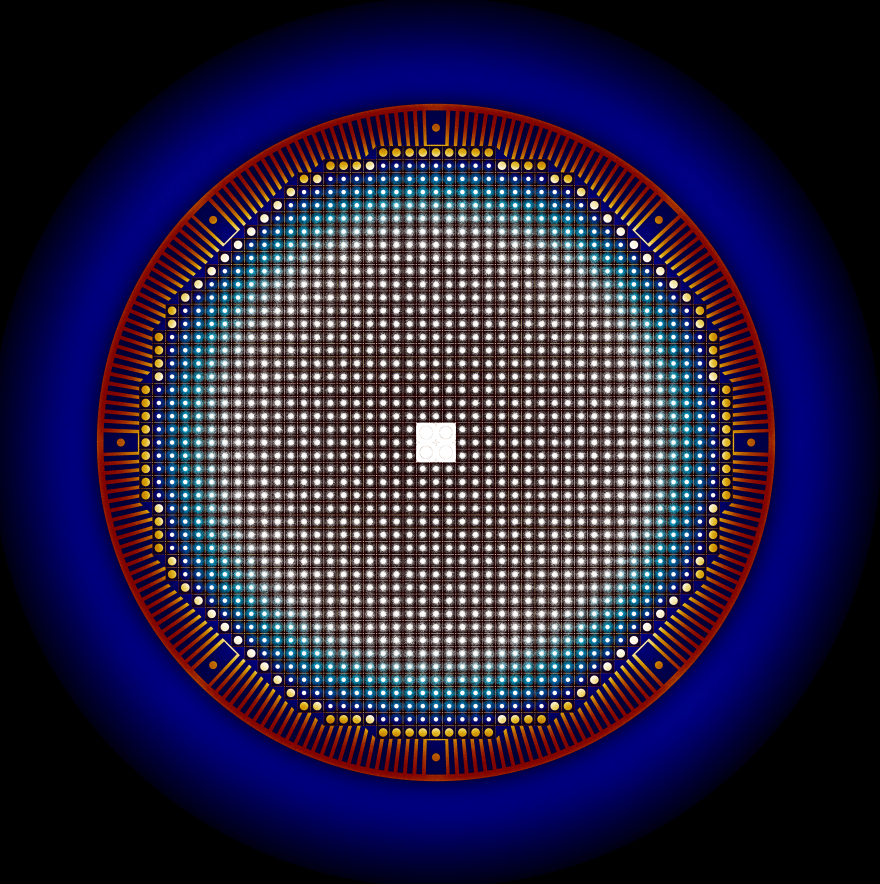
\includegraphics[width = \textwidth]{img/multiphysics.png}
                \vfill
            \end{tcolorbox}
        \end{minipage}
        \begin{minipage}{.3\linewidth}
            \begin{tcolorbox}[colback=white, colframe=black, width=\linewidth, height=1.35\linewidth, boxrule=1pt]
                \researcharea{Nuclear Fuel Cycle Analysis}
                \newline\vfill
                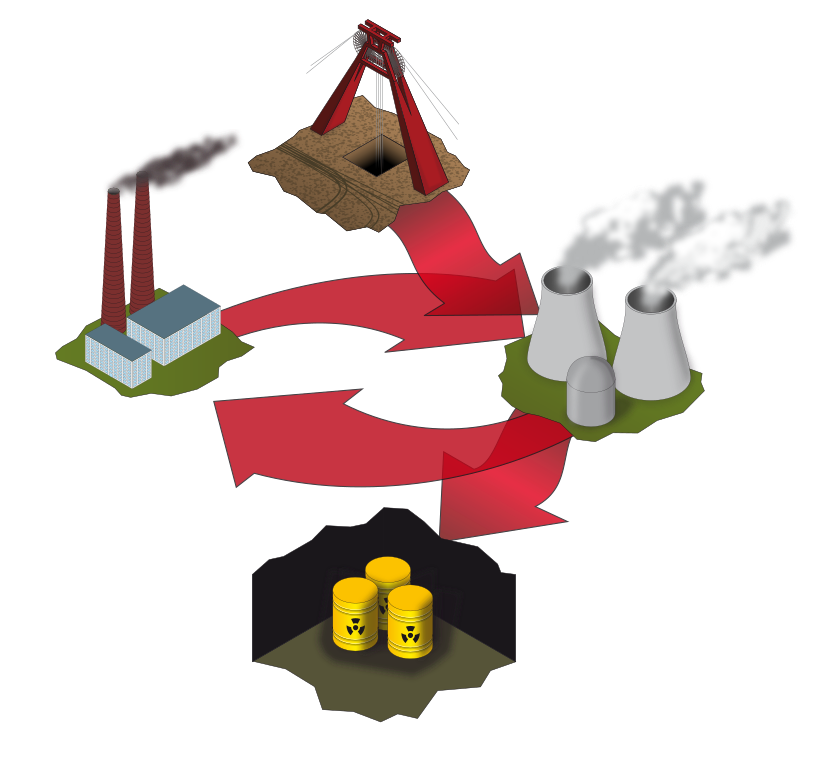
\includegraphics[width=\textwidth]{img/nfc.png}
                \vfill
            \end{tcolorbox}
        \end{minipage}
        \begin{minipage}{.3\linewidth}
            \begin{tcolorbox}[colback=white, colframe=black, width=\linewidth, height=1.35\linewidth, boxrule=1pt]
                \researcharea{Advanced Computation}
                \newline\vfill
                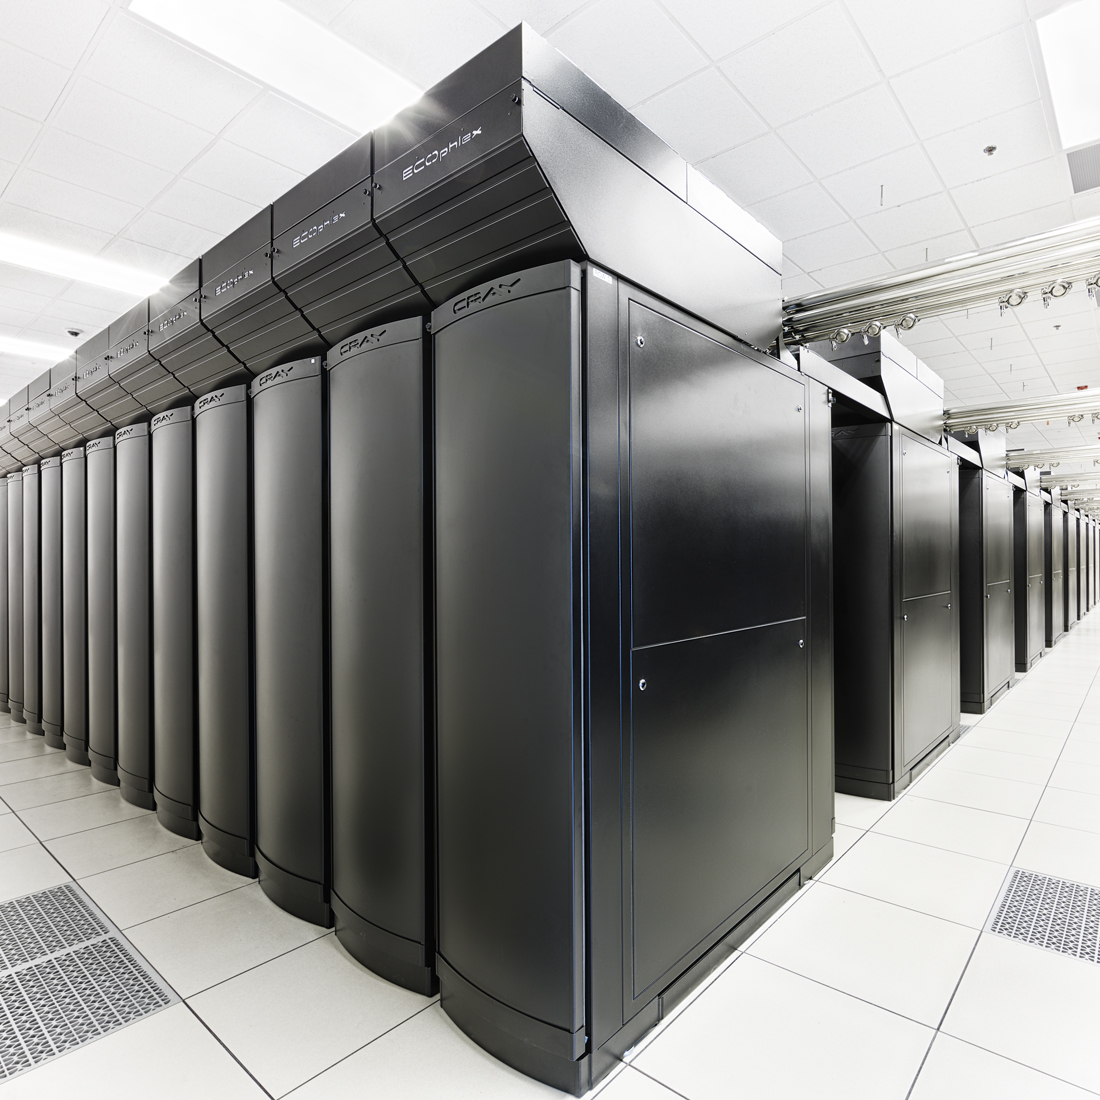
\includegraphics[width=\textwidth]{img/bw_cropped.jpg}
                \vfill
            \end{tcolorbox}
        \end{minipage}
    }

    %%%%%%%%%%%%%%%%%%%%%%%%%
    %%%% Logos of codes %%%%%
    %%%%%%%%%%%%%%%%%%%%%%%%%
    % \begin{tikzpicture}
    % \node (logos) [blurb, yshift = -19cm, xshift = -3cm] {\vspace{5pt}
    % \textcolor{black}{
    % \newline{\fontsizetitle Open-Source Nuclear Research Codes}\\
    % \vspace{-20pt}\rule{\textwidth}{5pt}\\
    % \vspace{25pt}
    % \begin{minipage}{.2\linewidth}
    %     
\includegraphics[width = \linewidth]{img/openmc_logo.png}\\
    %     \vspace{5pt}
    %     
\includegraphics[width = \linewidth]{img/rollo-logo.png}
    % \end{minipage} 
    % \begin{minipage}{.2\linewidth}
    %     
\includegraphics[width =.8\linewidth]{img/pyne.png}
    %     \vspace{10pt}
    % \end{minipage}
    % \begin{minipage}{.2\linewidth}
    %     
\includegraphics[width=.8\linewidth]{img/ghastly.png}
    % \end{minipage}
    % \begin{minipage}{.2\linewidth}
    %     
\includegraphics[width=\linewidth]{img/cyclus.png}\\
    %     \vspace{20pt}
    %     \textcolor{altgeldorange!100}{\textbf{\fontsizemoltres{\texttt{Moltres}}}}\\\vspace{-15pt}
    % \end{minipage}
    % }
    % };
    % \end{tikzpicture}

    %%%%%%%%%%%%%%%%%%%%%%%%%
    %%% Collaborator logos %%
    %%%%%%%%%%%%%%%%%%%%%%%%%
    % \vspace{1.5cm}
    % \begin{minipage}{.235\linewidth}
    %     \centering
    %     
\includegraphics[width=.8\linewidth]{img/qrcode.eps}
    %     \href{https://arfc.github.io/}{\fontsizesection\underline{https://arfc.github.io/}}
    % \end{minipage}
    % \vspace{-1cm}
    % \begin{minipage}{0.72\linewidth}
    %     \hspace{.5cm}
    %     \begin{tikzpicture}
    %     \vspace{-1cm}
    %         \node (logos) [blurb] {
    %         \begin{minipage}{.3\linewidth}
    %         `   %https://www.energy.gov/department-energy-logo-and-branding-guidelines
    %             
\includegraphics[width = \linewidth]{img/doe.png}
    %         \end{minipage}
    %         \begin{minipage}{.3\linewidth}
    %             %https://commons.wikimedia.org/wiki/File:NNSA_Logo.png
    %             
\includegraphics[width = \linewidth]{img/nnsa.png}
    %         \end{minipage}
    %         \begin{minipage}{.3\linewidth}
    %             % top left https://en.m.wikipedia.org/wiki/File:US-NuclearRegulatoryCommission-Logo.svg
    %             
\includegraphics[width = \linewidth]{img/nrc.png}
    %         \end{minipage}
    %         \vspace{1cm}
    %         \begin{minipage}{.3\linewidth}
    %         `   %https://www.moltexenergy.com/partners/ornl-logo/
    %             
\includegraphics[width = \linewidth]{img/ornl.png}
    %         \end{minipage}
    %         \begin{minipage}{.3\linewidth}
    %             %https://commons.wikimedia.org/wiki/File:Argonnelablogo.PNG
    %             
\includegraphics[width = \linewidth]{img/anl.png}
    %         \end{minipage}
    %         \begin{minipage}{.3\linewidth}
    %         \hspace{3.25cm}
    %             % https://inl.gov/logos-videos-images/
    %             
\includegraphics[height = .5\linewidth]{img/inl.png}
    %         \end{minipage}
    %         };
    %     \end{tikzpicture}
    % \end{minipage}

    %%%%%%%%%%%%%%%%%%%%%%%%%
    %%%%%% References %%%%%%%
    %%%%%%%%%%%%%%%%%%%%%%%%%
    \vspace{2cm}
    \begin{tcolorbox}[colback=white, colframe=black, width=0.9\textwidth, arc=6pt, boxrule=1pt]
        \bibliographystyle{plain}
        \bibliography{group-poster}
    \end{tcolorbox}
\end{center}
}{
}
}{
    \begin{center}
    %%%%%%%%%%%%%%%%%%%%%%%%%%%%%%%%%
    %%%%%%%%%%%% Moltres %%%%%%%%%%%%
    %%%%%%%%%%%%%%%%%%%%%%%%%%%%%%%%%
    \begin{tcolorbox}[colback=white, colframe=black, width=0.95\textwidth, arc=6pt, boxrule=1pt]
        \sectiontitle{Moltres}
        \sectioncontent{
            $S_N-D$ method for accurate time-dependent control rod modeling in Moltres,
            an open-source MOOSE application for the simulation of molten salt reactors \cite{park}.

            \includegraphics[width = .4\textwidth]{img/msre-full-0-power.png}
            \hspace{2cm}
            \includegraphics[width = .4\textwidth]{img/msre-full-123-power.png}
            
            \figcaption{
                    MSRE full core scalar flux error as calculated with pure diffusion, $S_N-D$,
                    and OpenMC for all control rods removed (left) and all control rods inserted (right)
            }
        }
    \end{tcolorbox}

    %%%%%%%%%%%%%%%%%%%%%%%%%%%%%%%%
    %%%%%%%%% OpenMCyclus %%%%%%%%%%
    %%%%%%%%%%%%%%%%%%%%%%%%%%%%%%%%
    \begin{tcolorbox}[colback=white, colframe=black, width=0.95\textwidth, arc=6pt, boxrule=1pt]
        \sectiontitle{OpenMCyclus}
        \sectioncontent{
            Reactor-physics informed fuel cycle analysis on the impacts of deploying HALEU-fueled reactors 
            using OpenMCyclus, a coupling of OpenMC with Cyclus \cite{bachmann}.

            \begin{minipage}{.45\textwidth}
                \vspace{1em}
                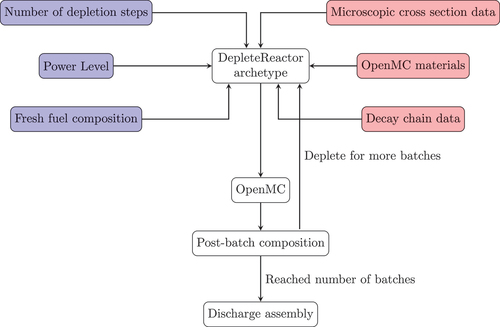
\includegraphics[width = \textwidth]{img/bachmann.jpg}
                \newline
                \figcaption{
                    Depletion methodology in OpenMCyclus. Blue comes from Cyclus and Red is 
                    provided through user-inputs.
                }
            \end{minipage}
            \hspace{1cm}
            \begin{minipage}{.45\textwidth}
                \vspace{1em}
                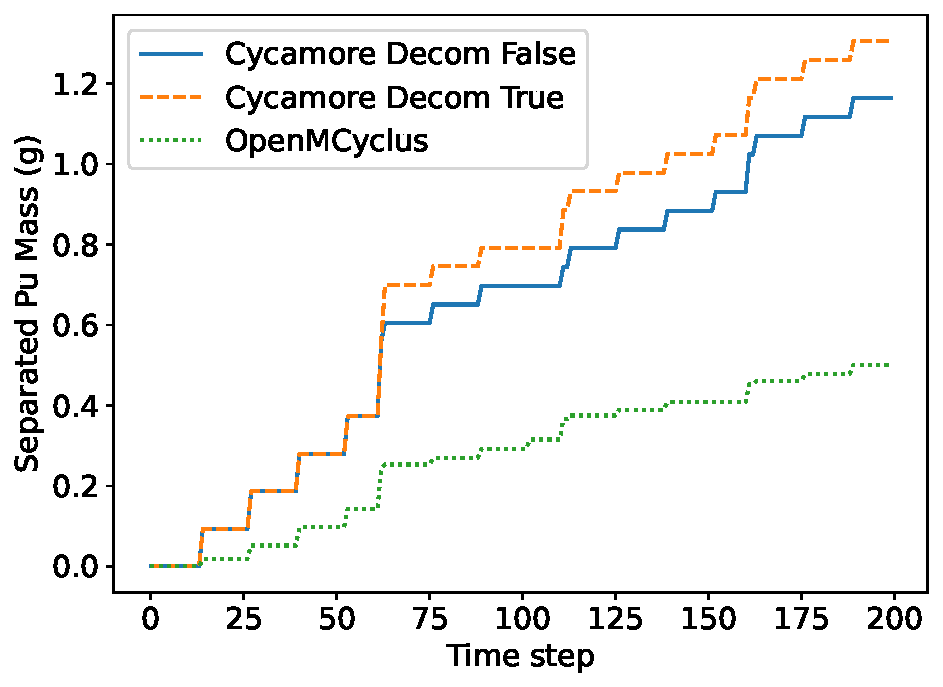
\includegraphics[width = \textwidth]{img/comparison_pu_cumulative.pdf}
                \newline
                \figcaption{
                    Comparison of the cumulative mass of separated plutonium traded after 
                    using the OpenMCyclus and Cycamore reactor.
                }
            \end{minipage}
        }
    \end{tcolorbox}

    %%%%%%%%%%%%%%%%%%%%%%%%%%%%%%%%%
    %%%%%%%%%%%%% ROLLO %%%%%%%%%%%%%
    %%%%%%%%%%%%%%%%%%%%%%%%%%%%%%%%%
    \begin{tcolorbox}[colback=white, colframe=black, width=0.95\textwidth, arc=6pt, boxrule=1pt]
        \sectiontitle{ROLLO}
        \sectioncontent{
            Evolutionary algorithm techniques applied to optimize nuclear reactor design by coupling 
            nuclear software to the DEAP evolutionary algorithm driver \cite{chee}.

            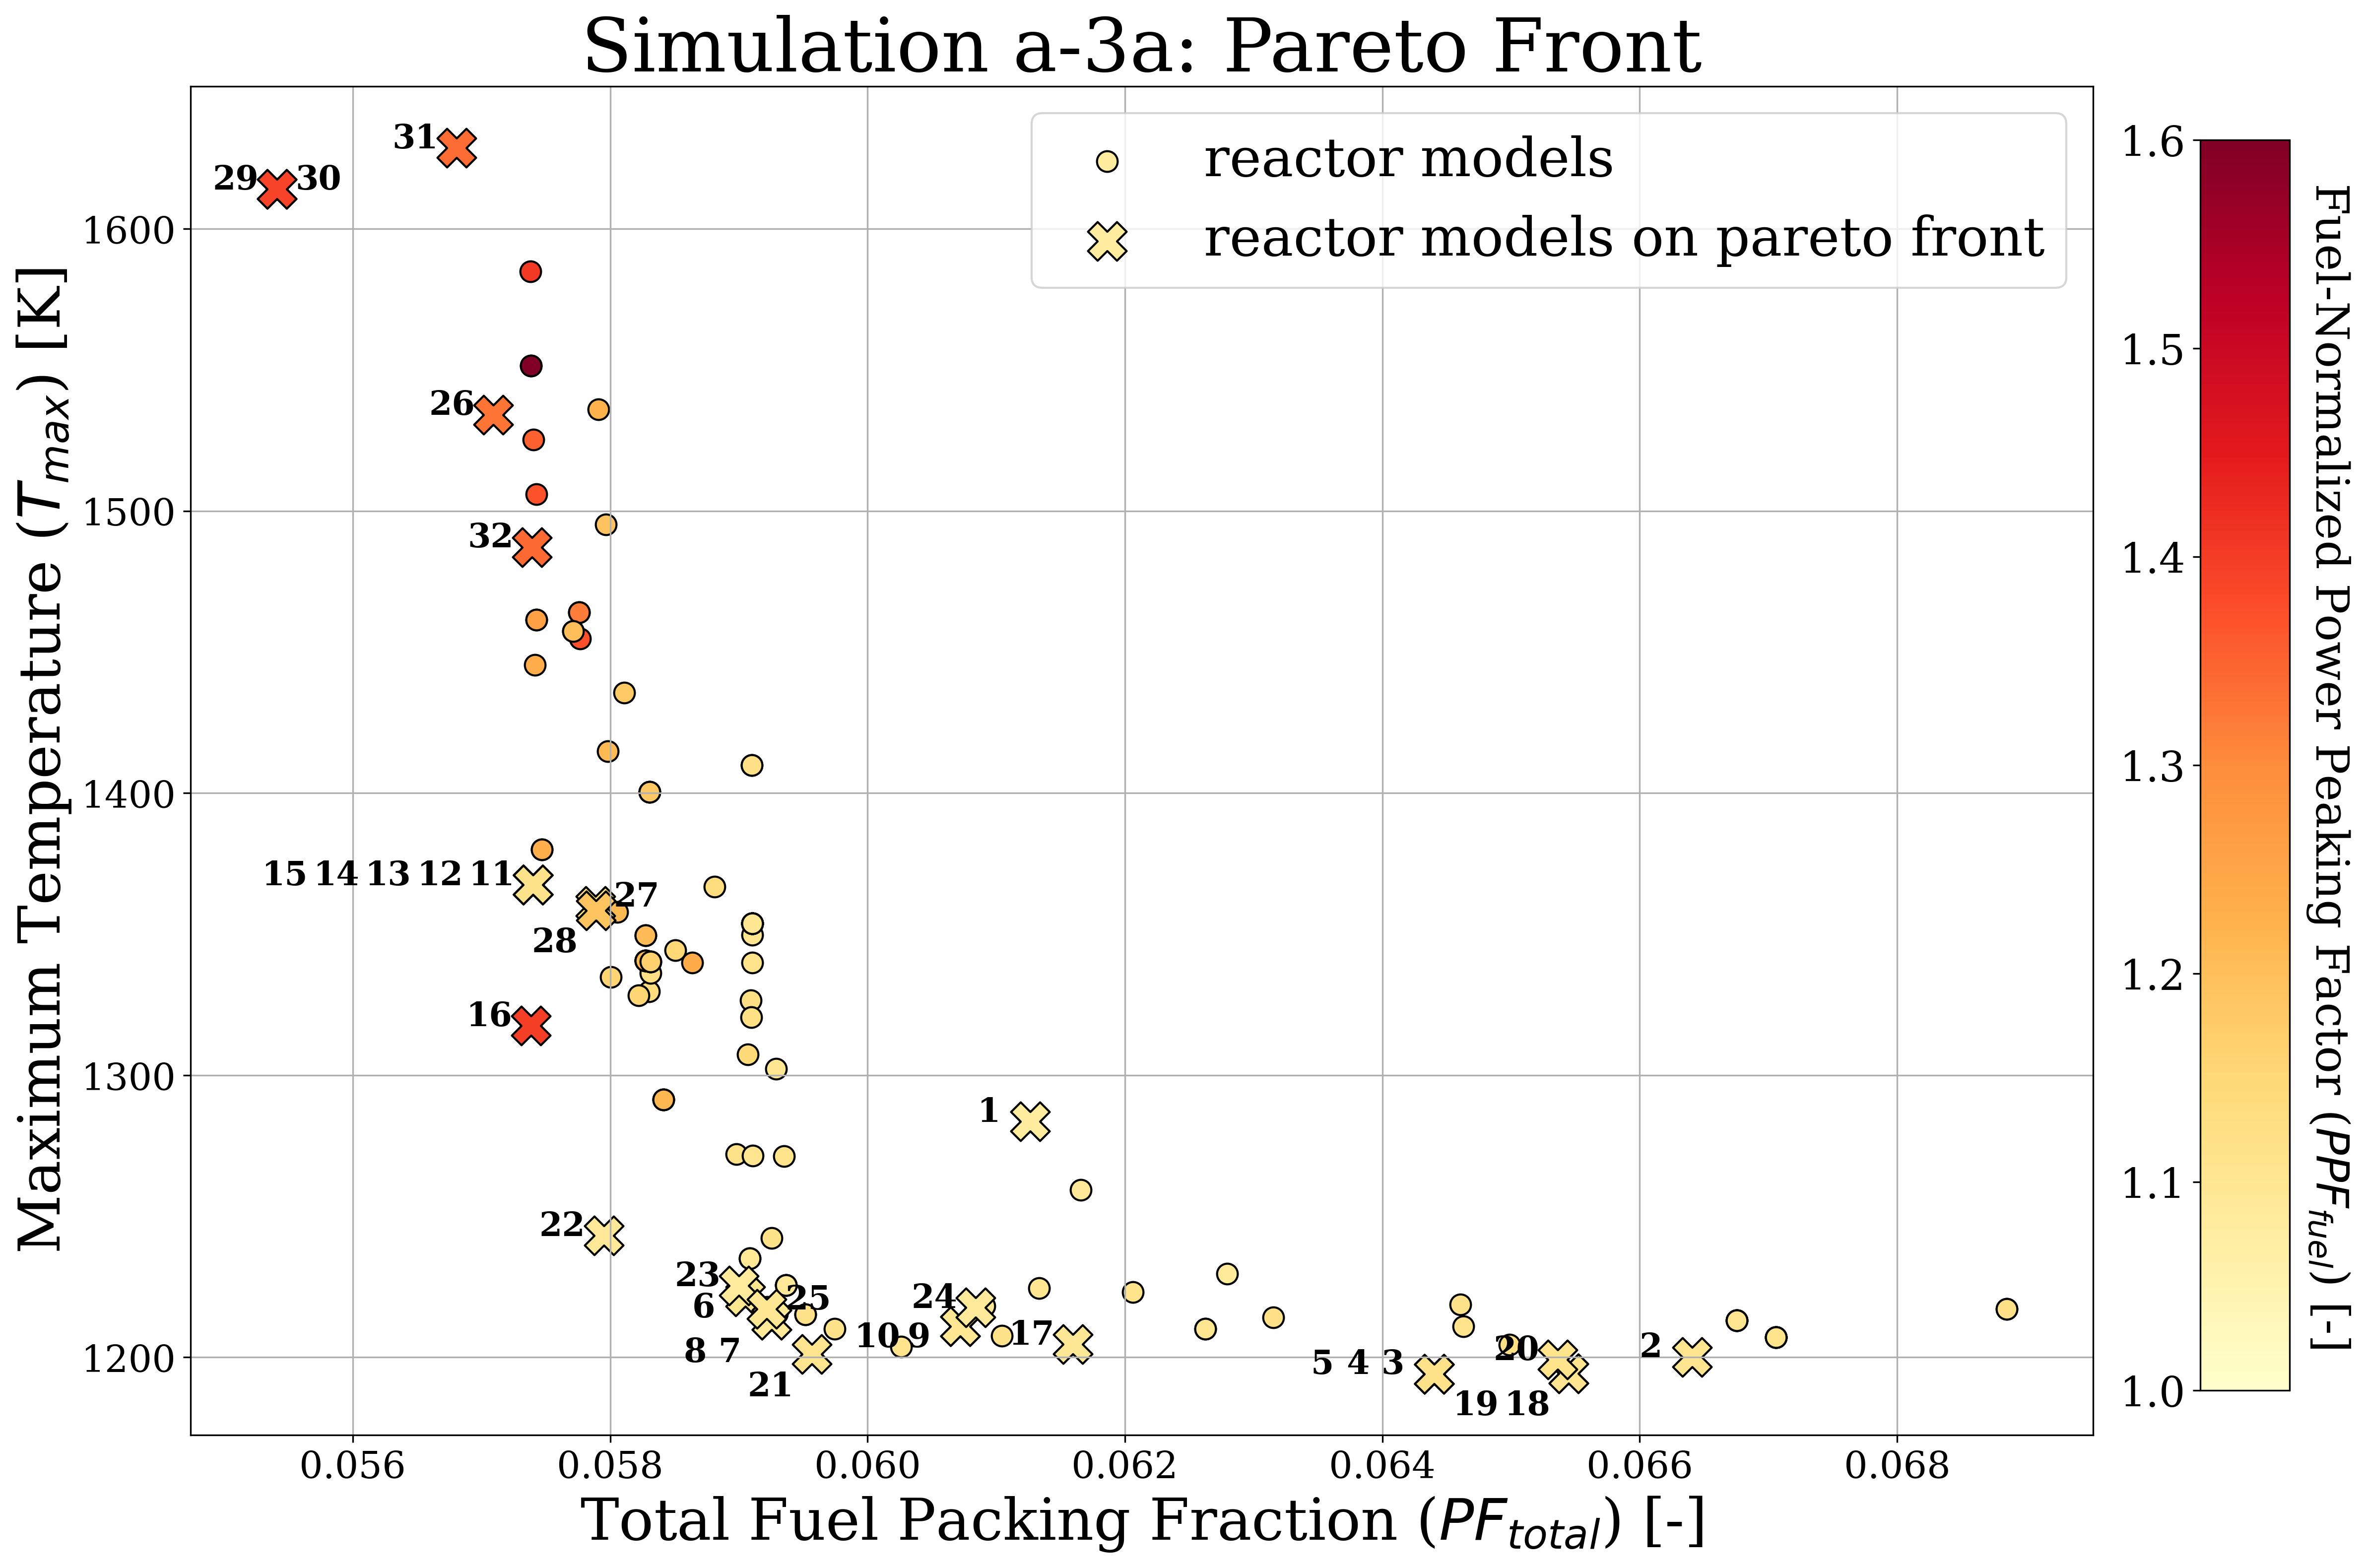
\includegraphics[width = .7\textwidth]{img/assem-obj-3-2d.png}
            \newline
            \figcaption{
                Triple-objective optimization to minimize total fuel packing fraction, max temp, and 
                fuel-normalized power peaking factor in the one-third assembly.
            }
        }
    \end{tcolorbox}

    %%%%%%%%%%%%%%%%%%%%%%%%%%%%%%%%%
    %%%%%% Logos (UIUC, ARFC) %%%%%%%
    %%%%%%%%%%%%%%%%%%%%%%%%%%%%%%%%%
    
\includegraphics[height=0.28\textwidth]{img/UIUC_Logo.png}\hspace{5cm}
    
\includegraphics[height=0.28\textwidth, trim={0 .5cm 0 .5cm}]{img/arfc_atom.png}

\end{center}
}{
    \vspace{-2.5cm}
\begin{tikzpicture}
    \node (physics) [blurb] {
    \vspace{5pt}
    \textcolor{black}{
    \newline{\fontsizetitle Physics of Advanced Reactors}\\
    \vspace{-20pt}\rule{\textwidth}{5pt}\\
    \fontsizesection
    Variance reduction methods for time-dependent Monte Carlo neutron transport. \\
        \vspace{20pt}
    Updated models of DNP group parameters for Molten Salt Reactors. \\
        \vspace{20pt}
    Computational modeling of flowing pebble-bed reactor systems.
        \begin{center}
        \begin{minipage}{.2\linewidth}
            
\includegraphics[height = 3\textwidth]{img/ghastly1.png}
        \end{minipage}
        \hspace{.5cm}
        \begin{minipage}{.2\linewidth}
            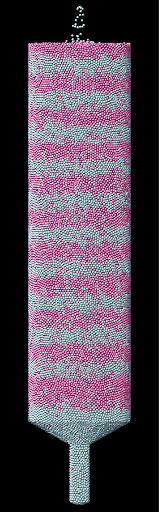
\includegraphics[height = 3\textwidth]{img/ghastly2.png}
        \end{minipage}
        \hspace{.5cm}
        \begin{minipage}{.2\linewidth}
            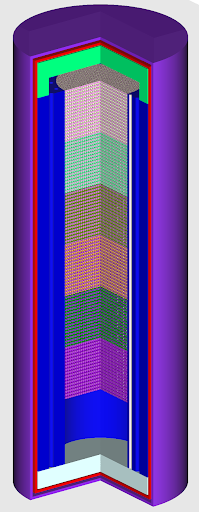
\includegraphics[height = 3\textwidth]{img/ghastly3.png}
        \end{minipage}
        \vspace{10pt}
        \figcaption{Simulation of a generic pebble bed HTGR core being filled (left) and online pebble recirculation (middle) using LAMMPS, 
        and a Xe-100-like full-core pebble bed HTGR (right) using SCALE \cite{richter}.}
        \end{center}
    }
    };
    \node (cycles) [blurb, below of = physics, yshift = -35.70cm] {
    \vspace{5pt}
    \textcolor{black}{
    \newline{\fontsizetitle Fuel Cycle and Energy System Optimization}\\
    \vspace{-20pt}\rule{\textwidth}{5pt}\\
    \fontsizesection
    Modeling and simulating scaled isotopic consequences of deploying Accelerators Driven Systems.\\
        \vspace{20pt}
    Techno-economic analysis of hybrid nuclear renewable energy systems (e.g. hydrogen microgrids).
        \begin{center}
        \begin{minipage}{.7\textwidth}
            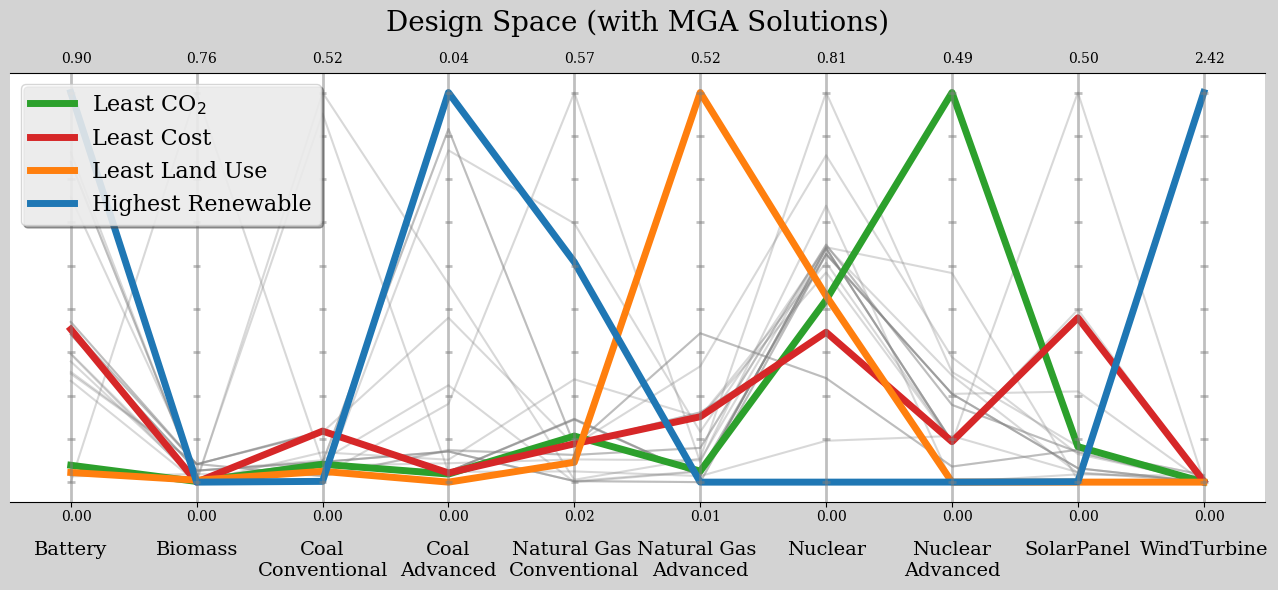
\includegraphics[width = \textwidth]{img/osier.png}
        \end{minipage}
        \vspace{10pt}
        \figcaption{The design space for a four objective problem including alternative solutions suggested by MGA.}
        \end{center}
        \vspace{20pt}
    Fuel cycle transition scenarios for advanced reactors.
        \begin{center}
        \begin{minipage}{.6\textwidth}
            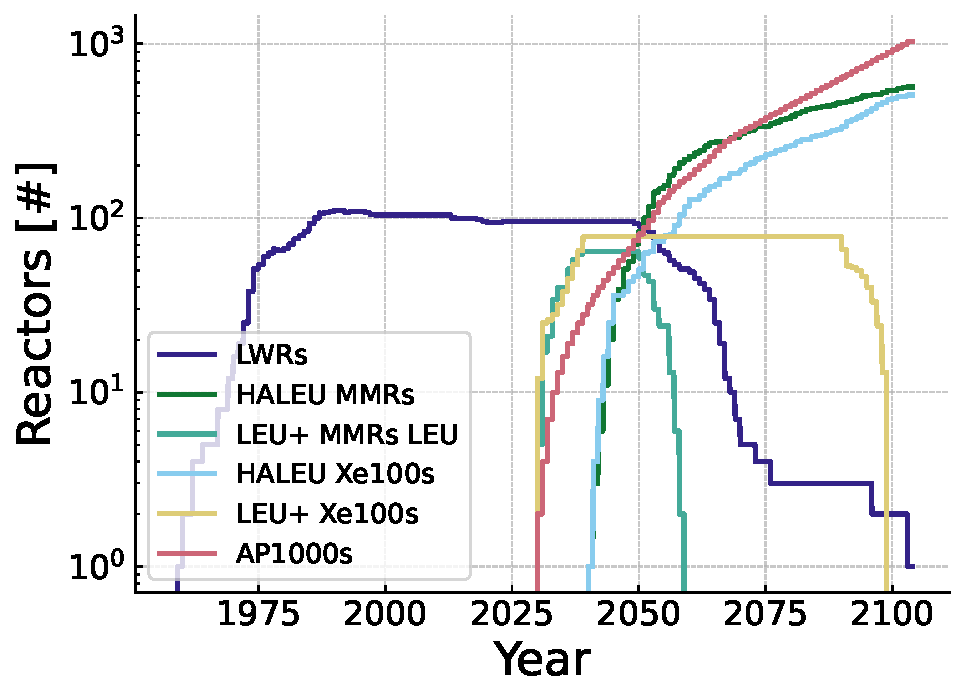
\includegraphics[width = \textwidth]{img/multi_dg2_reactors.pdf}
        \end{minipage}
        \vspace{10pt}
        \figcaption{Greedy AP1000 deployment along with Xe-100s and MMRs fueled by LEU+ and HALEU fuel.}
        \end{center}
    }
    };
\end{tikzpicture}
}
\end{document}
